\section{Exercises}

\exercise{1}{chapter-crl}{Design the \ttt{boolean isStrictlyIncreasing(int x, int y, int z)} that determines if three integers $x$, $y$, and $z$ are strictly increasing. By this, we mean that $x < y < z$.}

\exercise{1}{chapter-crl}{Design the \ttt{String numStuff(int n)} that determines if an integer $n$ is greater than $100$. If so, return the string of $n$ divided by two. If the number is less than 50, return the string of $n$ divided by five. In any other case, return the string ``N/A.''}

\exercise{1}{chapter-crl}{Design the \ttt{boolean canVote(int age)} that, when given an integer variable \emph{age} in years, returns whether or not someone who is that age is able to legally vote in the United States. For reference, someone may legally vote once they turn eighteen years old.}

\exercise{1}{chapter-crl}{Design the \ttt{int max(int x, int y, int z)} that returns the maximum of three integers $x$, $y$, and $z$. Do not use any built-in (\ttt{Math} library) methods.}

\exercise{1}{chapter-crl}{Design the \ttt{int computeRoundSum(int x, int y, int z)} method that computes the sum of the rounded values of three integers $x$, $y$, and $z$. By ``rounded values,'' we mean that we round their least significant digit, i.e., the rightmost digit either up or down depending on its value. For instance, 12 rounds down to 10, 59 rounds up to 60, and 1009 rounds up to 1010. If the number is negative, round towards zero when necessary, e.g., $-7$ rounds down to $-10$, $-2$ rounds up to zero.}

\exercise{1}{chapter-crl}{Design the \ttt{boolean lessThan20(int x, int y, int z)} method that, when given three integers $x$, $y$, and $z$, returns whether or not one of them is less than twenty away from another. For example, \ttt{lessThan20(19, 2, 412)} returns true because $2$ is less than $20$ away from $19$. Another example is \ttt{lessThan20(999, 888, 777)}, which returns false because none of the numbers have a difference less than twenty.}

\exercise{1}{chapter-crl}{Design the \ttt{boolean canSleepIn(String d, boolean onVacation)} method, which determines whether or not someone can sleep in. Someone is able to sleep in if it is a weekend or they are on vacation. The input $d$ is passed as a day of the week, e.g., \ttt{"Monday"}, ..., \ttt{"Sunday"}.}

\exercise{1}{chapter-crl}{Design the \ttt{boolean isEvenlySpaced(int x, int y, int z)} method, which receives three integers $x$, $y$, and $z$, and returns whether they are evenly spaced. Evenly spaced means that the difference between the smallest and medium number is the same as the difference between the medium and largest number.}

\exercise{1}{chapter-crl}{Design the \ttt{String cutTry(String s)} method, which receives a string $s$ and, if $s$ ends with \ttt{"try"}, it is removed. Otherwise, the original string is returned.}

\exercise{1}{chapter-crl}{Design the \ttt{String popChars(String s, char c, char d)} method, which receives a string $s$ and two characters $c, d$. The method removes $c$ if $s$ starts with $c$, and removes $d$ if the second character of $s$ is $d$. The remainder of the string is the same.}

\exercise{1}{chapter-crl}{Design the \ttt{String middleString(String a, String b, String c)} method, which receives three strings $a$, $b$, and $c$, and returns the string that is ``in between'' the others in terms of their lexicographical content. You cannot sort the strings or use an array.}

\exercise{1}{chapter-crl}{In propositional logic, there are several \emph{connectives} that act on boolean truth values. These include logical conjunction $\land$, disjunction $\lor$, conditional $\to$, biconditional $\leftrightarrow$, and negation $\lnot$. We can represent \emph{schemata} as a series of composed method calls. For example, an evaluation of}

\[
    `P \to \lnot (Q \leftrightarrow \lnot R)\textrm'
\]

\noindent where `$P$' and `$R$' are assigned to \ttt{false} and `$Q$' is assigned to \ttt{true}, is equivalent to

\begin{verbnobox}[\small]
static final boolean P = false;
static final boolean Q = true;
static final boolean R = false;

cond(P, not(bicond(Q, not(R))))
\end{verbnobox}

\noindent The presented schema resolves to \ttt{true}.

\noindent Design methods for the five connectives according to the following truth tables. These methods should be called \ttt{cond}, \ttt{bicond}, \ttt{and}, \ttt{or}, and \ttt{not}. Assume that $\mathrm{T}$ is \ttt{true} and $\mathrm{F}$ is \ttt{false}.
\captionsetup[subfigure]{labelformat=empty}
\captionsetup[figure]{labelformat=empty}%
\begin{figure}[H]
\begin{center}
    \begin{tabular}{c|c}
         $P$&$\lnot{P}$\\
         \hline
         $\mathrm{T}$&$F$\\
         $\mathrm{F}$&$\mathrm{T}$
    \end{tabular}
\end{center}
\caption{Truth Table of `$\lnot{P}$'}
\label{fig:ttnotp}
\end{figure}

\begin{figure}[H]
\begin{subfigure}{.5\textwidth}
\begin{center}
    \begin{tabular}{cc|c}
         $P$&$Q$&$P \land {Q} $\\
         \hline
         $\mathrm{T}$&$\mathrm{T}$&$\mathrm{T}$\\
         $\mathrm{T}$&$\mathrm{F}$&$\mathrm{F}$\\
         $\mathrm{F}$&$\mathrm{T}$&$\mathrm{F}$\\
         $\mathrm{F}$&$\mathrm{F}$&$\mathrm{F}$
    \end{tabular}
\end{center}
\caption{Truth Table of `$P \land Q$'.}
\label{fig:ttpandq}
\end{subfigure}
\begin{subfigure}{.5\textwidth}
\begin{center}
    \begin{tabular}{cc|c}
         $P$&$Q$&$P\lor{Q} $\\
         \hline
         $\mathrm{T}$&$\mathrm{T}$&$\mathrm{T}$\\
         $\mathrm{T}$&$\mathrm{F}$&$\mathrm{T}$\\
         $\mathrm{F}$&$\mathrm{T}$&$\mathrm{T}$\\
         $\mathrm{F}$&$\mathrm{F}$&$\mathrm{F}$
    \end{tabular}
\end{center}
\caption{Truth Table of `$P \lor Q$'.}
\label{fig:ttporq}
\end{subfigure}
\end{figure}

\begin{figure}[H]
\begin{subfigure}{.5\textwidth}
\begin{center}
    \begin{tabular}{cc|c}
         $P$&$Q$&$P\to{Q} $\\
         \hline
         $\mathrm{T}$&$\mathrm{T}$&$\mathrm{T}$\\
         $\mathrm{T}$&$\mathrm{F}$&$\mathrm{F}$\\
         $\mathrm{F}$&$\mathrm{T}$&$\mathrm{T}$\\
         $\mathrm{F}$&$\mathrm{F}$&$\mathrm{T}$
    \end{tabular}
\end{center}
\caption{Truth Table of `$P \to Q$'.}
\label{fig:ttptoq}
\end{subfigure}
\begin{subfigure}{.5\textwidth}
\begin{center}
    \begin{tabular}{cc|c}
         $P$&$Q$&$P\liff{Q} $\\
         \hline
         $\mathrm{T}$&$\mathrm{T}$&$\mathrm{T}$\\
         $\mathrm{T}$&$\mathrm{F}$&$\mathrm{F}$\\
         $\mathrm{F}$&$\mathrm{T}$&$\mathrm{F}$\\
         $\mathrm{F}$&$\mathrm{F}$&$\mathrm{T}$
    \end{tabular}
\end{center}
\caption{Truth Table of `$P \liff Q$'.}
\label{fig:ttpiffq}
\end{subfigure}
\end{figure}

\captionsetup[subfigure]{labelformat=simple}
\captionsetup[figure]{labelformat=simple}%

\exercise{1}{chapter-crl}{Design the \ttt{boolean isInsideCircle(double cx, double cy, double r, double px, double py)} method that, when given a circle centered at $(c_x, c_y)$ and radius $r$ as well as a point at $(p_x, p_y)$, returns whether the point is located strictly inside the circle.}

\exercise{1}{chapter-crl}{Design the \ttt{boolean isInsideRectangle(double rx, double ry, double w, double h, double px, double py)} method that, when given a rectangle centered at $(r_x, r_y)$, width $w$ and height $h$ as well as a point $(p_x, p_y)$, returns whether the point is located strictly inside the rectangle.}

\exercise{2}{chapter-crl}{Carlo is shipping out orders of candy to local grocery stores. Boxes have a maximum weight defined by a value $w$, and we can (potentially) fit both small and large bars of candy in a box. Design the \ttt{int fitCandy(int s, int l, int w)} method that, when given a number of small bars $s$, large bars $l$, and maximum weight $w$, determines the number of small candy bars he can fit in the box. Large bars weigh five kilograms, and small bars weigh one kilogram. Note that Carlo always tries to fit large candies first before small. Return \ttt{-1} if it is impossible to fill the box with the given criteria. Below are some test examples. Hint: consider this as an analysis of three cases.}

\begin{verbnobox}[\small]
fitCandy(4, 1, 9)      => 4
fitCandy(4, 1, 4)      => 4
fitCandy(1, 2, 6)      => 1
fitCandy(6, 1, 13)     => -1
fitCandy(60, 100, 550) => 50
fitCandy(7, 1, 12)     => 7
fitCandy(7, 1, 13)     => -1
\end{verbnobox}

\exercise{3}{chapter-crl}{An IPv4 address contains four integer values stored in four octets, separated by dots. For instance, \ttt{192.168.1.244} is a valid IPv4 address. Another example is \ttt{149.165.192.52}. Design the \ttt{boolean isValidIpv4(String ip)} method that, when given a string, determines whether or not it represents a valid IPv4 address. Each octet must be an integer between zero and 255 inclusive. Note that some IPv4 addresses are, in reality, nonsensical, e.g., \ttt{0.0.0.0}, but we will not consider these as invalid. Below the examples is a helper method, \ttt{isNumeric}, to determine whether or not a string is ``numeric.'' Understanding \emph{how} this helper method works is unimportant for the time being. You \textbf{cannot} use arrays, loops, or regular expressions to solve this problem. Finally, you will need to use \ttt{Integer.parseInt}, \ttt{substring}, and \ttt{indexOf}.}

\begin{verbnobox}[\small]
isValidIpv4("192.168.1.244")    => true
isValidIpv4("149.165.192.52")   => true
isValidIpv4("192.168.1.256")    => false
isValidIpv4("192.168.1201.23")  => false
isValidIpv4("192.168.1201.ABC") => false
isValidIpv4("ABC.DEF.GHI")      => false
isValidIpv4("192.168.1A6.201")  => false
\end{verbnobox}

\begin{lstlisting}[language=MyJava]
/**
 * Determines whether or not we can convert a given string into 
 * an integer datatype.
 * @param n - input string.
 * @return true if the string is convertable to an integer, false otherwise.
 */
static boolean isNumeric(String n) {
  try {
    Integer.parseInt(n);
    return true;  
  } catch (NumberFormatException ex) {
    return false;
  }
}
\end{lstlisting}

\exercise{1}{chapter-crl}{Design the \ttt{String stateOfMatter(double t, char u)} method that receives a water temperature as a \ttt{double} and a unit as a \ttt{char}, i.e., either \ttt{`C'} or \ttt{`F'} for Celsius and Fahrenheit respectively. Return a string representing whether the water is a liquid, solid, or gas at sea level.}

\exercise{1}{chapter-crl}{Design the \ttt{double computeGpa(String grade)} method that translates a letter grade into a number grade. Letter grades are A, B, C, D, and F, possibly followed by + or -. Their numeric values are 4, 3, 2, 1, and 0. There is no F+ or F-. A+ increases the numeric value by 0.3, a - decreases it by 0.3. However, an A+ has value 4.0.}

\exercise{1}{chapter-crl}{Design the \ttt{String sortThreeStrings(String a, String b, String c)} method that receives three strings and sorts them lexicographically. Return the sorted set of strings as a string itself, separated by commas. For example, if the input is \ttt{Charlie}, \ttt{Able}, \ttt{Baker}, you should return \ttt{Able,Baker,Charlie}.}

\exercise{1}{chapter-crl}{Design the \ttt{int trickSum(int x, int y, int z)} method that sums the three integer inputs. If one of those values is $17$, however, it and any numbers to its right should not be included in the sum. For example, \ttt{trickSum(13, 17, 3)} resolves to \ttt{13} because, when $y=\ttt{17}$, we add neither $y$ nor $z$ to the resulting sum.}

\exercise{1}{chapter-crl}{A year with $366$ days is called a leap year. Leap years are necessary to keep the calendar synchronized with the sun because the earth revolves around the sun once every $365.25$ days. Actually, that figure is not entirely precise, and for all dates after $1582$ the Gregorian correction applies. Usually years that are divisible by 4 are leap years, for example $1996$. However, years that are divisible by $100$ (for example, $1900$) are not leap years, but years that are divisible by $400$ are leap years (for example, $2000$). Design the \ttt{boolean isLeapYear(int y)} method that receives a year (as an integer) $y$ and computes whether $y$ is a leap year. Use a single \ttt{if} statement and Boolean operators.}

\exercise{1}{chapter-crl}{Design the \ttt{double computeDiscount(double c, int age, boolean isStudent)} met\-hod that computes a discount for some item cost $c$ based on their age $\mathit{age}$ and student status according to the following criteria:}
\begin{itemize}
    \item If $\mathit{age} < 18$, apply a $20\%$ discount.
    \item If $18 \leq \mathit{age} \leq 25$ and they are a student, apply a $25\%$ discount. If they are not a student, do not apply a discount.
    \item If $\mathit{age} \geq 65$ and they are a student, apply a $30\%$ discount. If they are not a student, apply a $15\%$ discount.
    \item All other cases should not have a discount applied.
\end{itemize}
Your method should return the total cost of the item after applying the discount.

\exercise{1}{chapter-crl}{Design the \ttt{double computeTaxCost(double itemCost, String state)} method that computes the tax for some item based on the state in which it is purchased. The method should return the total cost of the item, which includes the taxed amount. The tax rates are as follows:}
\begin{itemize}
    \item \ttt{"CA"}: $9.25\%$
    \item \ttt{"NY"}: $4.0\%$
    \item \ttt{"NC"}: $6.625\%$
    \item \ttt{"SC"}: $6.0\%$
    \item \ttt{"VA"}: $6.25\%$
    \item \ttt{"WA"}: $6.5\%$
    \item \ttt{"IN"}: $8.0\%$
\end{itemize}

\exercise{1}{chapter-crl}{Design the \ttt{double computeOvertimePay(double hrRate, double noHrs, boolean onVacation, double taxRate)} method that computes the amount of overtime pay (note: \textbf{only} the overtime pay) given to an employee under the following conditions:}
\begin{itemize}
    \item An employee's base overtime pay rate is $1.5$ times their hourly rate.
    \item If the employee is on vacation, their pay rate is $2$ times their hourly rate rather than $1.5$.
    \item If the number of hours is less than or equal to $40$, then no overtime pay is given.
    \item If the number of hours is greater than $70$, then the resulting gross pay (before taxes) is increased by $15\%$.
    \item The gross pay is subject to the tax \emph{percentage} passed to the method. 
\end{itemize}

\exercise{1}{chapter-crl}{Design the \ttt{double computeBonusPay(double baseSalary, int yearsOfService, boolean achievedTarget, double salesAmount, double targetSales)} method that calculates the amount of bonus pay (note: \textbf{only} the bonus pay) given to an employee under the following conditions:}
\begin{itemize}
    \item A base bonus rate of $10\%$ of the base salary is given to employees who have achieved their sales target.
    \item Employees with more than $5$ years of service receive an additional $5\%$ bonus of their base salary.
    \item If the sales amount exceeds the target sales by more than $50\%$, the employee receives an additional bonus of $25\%$ of the base salary.
    \item If the employee has not achieved their sales target, they receive a flat bonus of $2\%$ of their base salary, regardless of sales amount or years of service.
    \item The total bonus amount is reduced by a flat tax rate of $25\%$.
\end{itemize}

\exercise{1}{chapter-crl}{Design the recursive \ttt{int countStr(String s)} that counts the number of times the substring \ttt{"str"} appears in a given string $s$.}

\exercise{1}{chapter-crl}{Rewrite the \ttt{countStr} method to use tail recursion. Name this new version of the method \ttt{countStrTR}. Hint: you will need to design a \ttt{private static} helper method. The \ttt{countStrTR} method should only have one parameter.}

\exercise{1}{chapter-crl}{Design the recursive \ttt{String replaceAB(String s)} method that replaces any occurrence of the character \ttt{`A'} with the character \ttt{`B'} in a given string $s$.}

\exercise{1}{chapter-crl}{Rewrite the \ttt{replaceAB} method to use tail recursion. Name this new version of the method \ttt{replaceABTR}. Hint: you will need to design a \ttt{private static} helper method. The \ttt{replaceABTR} method should only have one parameter.}

\exercise{1}{chapter-crl}{Elephants have two ears, right? Design the recursive \ttt{int countElephantEars(int n)} that returns the total number of elephant ears that are in a group of $n$ elephants.}

\exercise{1}{chapter-crl}{Rewrite the \ttt{countElephantEars} method to use tail recursion. Name this new version of the method \ttt{countElephantEarsTR}. Hint: you will need to design a \ttt{private static} helper method. The \ttt{countElephantEarsTR} method should only have one parameter.}

\exercise{1}{chapter-crl}{This question has two parts.}
\begin{enumerate}[label=(\alph*)]
    \item Design the \ttt{raiseLowerToUpperTR} tail recursive method, which receives a string and returns the number of lowercase characters raised to the number of uppercase characters, ignoring any other character. If there are no lowercase or uppercase characters, return zero. Hint: you will need to design a \ttt{private static} helper method to solve this problem.
    \item Design the \ttt{raiseLowerToUpperLoop} method that solves this problem using a loop.
\end{enumerate}
If you write tests for one of these methods, you should be able to propagate it through the other, so write plenty!


\exercise{2}{chapter-crl}{This question has two parts.}
\begin{enumerate}[label=(\alph*)]
    \item Design the \ttt{isPrimeTR} tail recursive method, which receives a positive integer and determines if it is prime. Recall that a number is prime if and only if it evenly divides only one and itself. Hint: you will need to design a \ttt{private static} helper method to solve this problem.
    \item Design the \ttt{isPrimeLoop} method that solves the problem using a loop.
\end{enumerate}

If you write tests for one of these methods, you should be able to propagate it through the other, so write plenty!

\exercise{1}{chapter-crl}{This question has two parts.}
\begin{enumerate}[label=(\alph*)]
    \item Design the \ttt{isPalindromeTR} tail recursive method, which receives a string and determines if it is a palindrome. Recall that a palindrome is a string that is the same backwards as it is forwards. E.g., ``racecar.'' \textbf{Do not} use a (character) array, \ttt{StringBuilder}, \ttt{StringBuffer}, or similar, to solve this problem. It \emph{must} be naturally recursive.
    \item Design the \ttt{isPalindromeLoop} method that solves the problem using a loop. The same restrictions from the previous problem hold true for this one.
\end{enumerate}

If you write tests for one of these methods, you should be able to propagate it through the other, so write plenty!

\exercise{1}{chapter-crl}{This question has two parts.}
\begin{enumerate}[label=(\alph*)]
    \item Design the \ttt{gcdTR} tail recursive method, which receives two integers and returns the greatest common divisor between the two. Euclid's algorithm is the basis for this approach and is a tail recursive algorithm by design.
    \item Design the \ttt{gcdLoop} method that solves the problem using a loop.

    If you write tests for one of these methods, you should be able to propagate it through the other, so write plenty!
\end{enumerate}

\exercise{1}{chapter-crl}{This question has two parts.}
\begin{enumerate}[label=(\alph*)]
    \item Design the \ttt{isNestedParenthesesTR} tail recursive method, which receives a string and determines if its parentheses pairs are ``balanced.'' A pair of parentheses is balanced if it is a nesting of zero or more pairs of parenthesis, like ``(())'' or ``((())).'' Note that pairs like ``(()())'' will not be tested.

    \item Design the \ttt{isNestedParenthesesLoop} method that solves the problem using a loop.
\end{enumerate}

If you write tests for one of these methods, you should be able to propagate it through the other, so write plenty!

\exercise{1}{chapter-crl}{This question has three parts.}

\begin{enumerate}[label=(\alph*)]
    \item The \emph{hyperfactorial} of a number, namely $H(n)$, is the value of $1^1 \cdot 2^2 \cdot ... \cdot n^n$. As you might imagine, the resulting numbers from a hyperfactorial are outrageously large. Therefore we will make use of the \ttt{long} datatype rather than \ttt{int} for this problem. 
    
    Design the standard recursive \ttt{hyperfactorial} method, which receives a long integer $n$ and returns its hyperfactorial.
    \item Then, design the \ttt{hyperfactorialTR} method that uses tail recursion and accumulators to solve the problem. Hint: you will need to design a \ttt{private static} helper method to solve this problem.

    \item Finally, design the \ttt{hyperfactorialLoop} method that solves the problem using a loop.
\end{enumerate}

If you write tests for one of these methods, you should be able to propagate it through the rest, so write plenty!

\exercise{1}{chapter-crl}{This question has three parts.}

\begin{enumerate}[label=(\alph*)]
    \item The \emph{subfactorial} of a number, namely $!n$, is the number of permutations of $n$ objects such that no object appears in its natural spot. For example, take the collection of objects $\{a, b, c\}$. There are $6$ possible permutations (because we choose arrangements for three items, and $3!=6$): $\{a, b, c\}, \{a, c, b\}, \{b, c, a\}, \{c, b, a\}, \{c, a, b\}, \{b, a, c\}$, but only two of these are \emph{derangements}: $\{b, c, a\}$ and $\{c, a, b\}$, because no element is in the same spot as the original collection. Therefore, we say that $!3=2$. We can describe subfactorial as a recursive formula:
\begin{align*}
    !0 &= 1\\
    !1 &= 0\\
    !n &= (n-1) \cdot (!(n - 1)\;+\;!(n - 2))
\end{align*}

    Design the standard recursive \ttt{subfactorial} method, which receives an long integer $n$ and returns its subfactorial. Because the resulting subfactorial values can grow insanely large, we will use the \ttt{long} datatype instead of \ttt{int}.

    \item Then, design the \ttt{subfactorialTR} method that uses tail recursion and accumulators to solve the problem. Hint: you will need to design a \ttt{private static} helper method to solve this problem.

    \item Finally, design the \ttt{subfactorialLoop} method that solves the problem using a loop.
\end{enumerate}

If you write tests for one of these methods, you should be able to propagate it through the rest, so write plenty!

\exercise{1}{chapter-crl}{This question has three parts.}
\begin{enumerate}[label=(\alph*)]
\item Design the standard recursive \ttt{collatz} method, which receives a positive integer and returns the Collatz sequence for said integer. This sequence is defined by the following recursive process:
\begin{align*}
    \ttt{collatz(1)} &= \ttt{1}\\
    \ttt{collatz(n)} &= \ttt{collatz(3 * n + 1)} \text{ if \ttt{n} is odd.}\\
    \ttt{collatz(n)} &= \ttt{collatz(n / 2)} \text{ if \ttt{n} is even.}
\end{align*}
The sequence generated is the numbers received by the method until the sequence reaches one (note that it is an open research question as to whether this sequence converges to one for every positive integer). So, \ttt{collatz(5)} returns the following \ttt{String} of comma-separated integers: \ttt{"5,16,8,4,2,1"}. \textbf{The last number cannot have a comma afterwards}.

\item Then, design the \ttt{collatzTR} method that uses tail recursion and accumulators to solve the problem. Hint: you will need to design a \ttt{private static} helper method to solve this problem.

\item Finally, design the \ttt{collatzLoop} method that solves the problem using a loop.
\end{enumerate}

If you write tests for one of these methods, you should be able to propagate it through the rest, so write plenty!

\exercise{1}{chapter-crl}{This question has three parts.}
\begin{enumerate}[label=(\alph*)]
\item Design the standard recursive \ttt{parenthesesDepth} method, which receives a string of parentheses and returns an integer representing the ``depth'' at the end of the string. Each instance of \texttt{(} increments the depth counter, and each instance of \texttt{)} decrements the depth counter. So, e.g., \texttt{"((())()))))(()"} is $1+1+1-1-1+1-1-1-1-1-1+1+1=-2$.

\item Then, design the \ttt{parenthesesDepthTR} method that uses tail recursion and accumulators to solve the problem. Hint: you will need to design a \ttt{private static} helper method to solve this problem.

\item Finally, design the \ttt{parenthesesDepthLoop} method that solves the problem using a loop.
\end{enumerate}

If you write tests for one of these methods, you should be able to propagate it through the rest, so write plenty!

\exercise{1}{chapter-crl}{This question has three parts.}
\begin{enumerate}[label=(\alph*)]
\item Design the standard recursive \ttt{countdown} method, which receives an \texttt{int} $n \geq 0$ and returns a \texttt{String} containing a sequence of the even numbers from $n$ down to $0$ inclusive, separated by commas.

\item Then, design the \ttt{countdownTR} method that uses tail recursion and accumulators to solve the problem. Hint: you will need to design a \ttt{private static} helper method to solve this problem.

\item Finally, design the \ttt{countdownLoop} method that solves the problem using a loop.
\end{enumerate}

If you write tests for one of these methods, you should be able to propagate it through the rest, so write plenty!

\exercise{2}{chapter-crl}{This question has three parts.}
\begin{enumerate}[label=(\alph*)]
    \item Design the standard recursive \ttt{chickenCounter} method, which receives a string $s$ and returns the number of times the substring \ttt{"chicken"} appears in $s$. You must account for overlapping instances of \ttt{"chicken"}. For example, calling the method with \ttt{"abcchickechickenn"} returns $2$ because, after removing the substring \ttt{"chicken"} from the original string, we are left with \ttt{"abcchicken"}, which itself contains another instance of \ttt{"chicken"}.

    \item Then, design the \ttt{chickenCounterTR} method that uses tail recursion and accumulators to solve the problem. Hint: you will need to design a \ttt{private static} helper method to solve this problem.

    \item Finally, design the \ttt{chickenCounterLoop} method that solves the problem using a loop.
\end{enumerate}

If you write tests for one of these methods, you should be able to propagate it through the rest, so write plenty!

\exercise{3}{chapter-crl}{This question has five parts. We need to provide some background for the question first. An \emph{encoded string} $S$ is one of the form:}
\begin{align*}
S &= G^{*}\\
G &= NL\\
N &= [\text{\ttt{0}---\ttt{9}}]^{+}\\
L &= [\text{\ttt{a}---\ttt{z}}]^{+}
\end{align*}
We imagine this didn't clear up what the definition means. Take the encoded string \ttt{"3[a]2[b]"} as an example. The resulting decoded string is \ttt{"aaabb"}, because we create three copies of \ttt{"a"}, followed by two copies of \ttt{"b"}. Another example is \ttt{"4[abcd]"}, which returns the string containing \ttt{"abcdabcdabcdabcd"}.

\begin{enumerate}[label=(\alph*)]
    \item First, design the \ttt{int retrieveN(String s)} that returns the integer at the start of an encoded string. Take the following examples as motivation.
\begin{verbatim}
retrieveN("3[a]2[b]")     => 3
retrieveN("47[abcd]")     => 47
retrieveN("1[bbbbb]3[a]") => 1
\end{verbatim}
    \item Next, design the \ttt{String cutN(String s)} method that returns a string without the integer at the start of an encoded string. Hint: use \ttt{indexOf} and \ttt{substring}.
\begin{verbatim}
cutN("3[a]2[b]")     => "[a]2[b]
cutN("47[abcd]")     => "[abcd]"
cutN("1[bbbbb]3[a]") => "[bbbbb]3[a]"
\end{verbatim}
    \item Design the \emph{standard recursive} \ttt{decode} method, which receives an encoded string and performs a decoding operation.
    \item Design the \texttt{decodeTR} and \texttt{decodeTRHelper} methods. The former acts as the driver to the latter; the latter solves the same problem that \texttt{decode} does, but it instead uses tail recursion. Remember to include the relevant access modifiers!
    \item Design the \texttt{decodeLoop} method, which solves the problem using either a \texttt{while} or \texttt{for} loop.
\end{enumerate}

\exercise{2}{chapter-crl}{Design the \ttt{boolean isNumberPalindrome(int n)} method that, when given an integer $n$, returns whether or not that number is a palindrome. You cannot convert the number to a string.}

\exercise{3}{chapter-crl}{The C programming language contains the \ttt{atoi} ``ascii-to-integer'' function, which receives a string and, if the string represents some integer, returns the number converted to an integer. Design the \ttt{int atoi(String s)} method that, when given a string $s$, returns its value as an integer if it can be parsed as an integer. When parsing the integer, ignore all leading zeroes and leading non-digits. Upon finding the first non-zero digit, if it exists, begin interpreting the string as a number. At any point thereafter, if a non-digit is encountered, return the number parsed up to that point. The given integer can also contain a sign, e.g., $+$ or $-$. If the value exceeds the bounds of an integer (i.e., \ttt{Integer.MAX_VALUE} or \ttt{Integer.MIN_VALUE}), return zero. Writing enough tests is \emph{crucial} to getting this correct! We provide some examples below.}

\begin{verbnobox}[\small]
atoi("ABCD")           => 0
atoi("42")             => 42
atoi("000042")         => 42
atoi("004200")         => 4200
atoi("ABCD42ABCD)      => 42
atoi("ABCD-+42ABCD)    => 42
atoi("ABCD+-42ABCD)    => -42
atoi("9999999999999")  => 0
atoi("-9999999999999") => 0
atoi("000-42000")      => -42000
atoi("000-ABCD)        => 0
atoi("000+42ABCD)      => 42
atoi("8080*8080)       => 8080
\end{verbnobox}

\exercise{3}{chapter-crl}{Similar to \ttt{atoi}, the C programming language also has a way of converting floating-point values represented as strings to double values via \ttt{atof}. Design the \ttt{double atof(String s)} method, which receives a string and converts it into a double if the input can be interpreted as such. To make this a bit easier, assume that only valid floating-point values can be passed to the method. Below are some examples. Due to potential inaccuracies with floating-point precision, as long as you are close to the given number, that is fine.}

\begin{verbnobox}[\small]
atof("3.1415")    => 3.1415
atof("+3.1415")   => -3.1415
atof("-3.1415")   => -3.1415
atof("100.0005")  => 100.0005
atof("6.28")      => 6.28
atof("3")         => 3.0
atof("0")         => 0.0
atof("-0.000000") => -0.000000
\end{verbnobox}

\exercise{2}{chapter-crl}{Design the \ttt{int indexOf(String s, String k)} method, which receives two strings $s$, $k$, and returns the first index of $k$ in $s$. Note that $k$ may be any arbitrary string and not just a a single character. If $k$ is not in $s$, return \ttt{-1}. You \textbf{cannot} use the \ttt{indexOf} method provided by the \ttt{String} class.}

\exercise{2}{chapter-crl}{Design the \ttt{String substring(String s, int a, int b)} method, which receives a string and two integers $a$, $b$, and returns the substring between these indices. If either are out of bounds of the string, return \ttt{null}. You \textbf{cannot} use the \ttt{substring} method(s) provided by the \ttt{String} class.}

\exercise{1}{chapter-crl}{Design the \ttt{boolean isEqualTo(String s1, String s2)} method, which receives two strings $s_1$ and $s_2$, and determines whether they are lexicographically equal. You cannot use the built-in \ttt{equals} or \ttt{compareTo} methods.}

\exercise{2}{chapter-crl}{Design the \ttt{int compareTo(String s1, String s2)} method that receives two strings $s_1$ and $s_2$, and compares their contents lexicographically. If \ttt{s1} is less than \ttt{s2}, return \ttt{-1}. If \ttt{s1} is greater than \ttt{s2}, return \ttt{1}. Otherwise, return \ttt{0}. Note that our implementation of \ttt{compareTo} will differ from Java's in that, if \ttt{s1} has less characters than \ttt{s2}, we return \ttt{-1}; if \ttt{s2} has less characters than \ttt{s1}, we return \ttt{1}. Otherwise, we do the character-by-character comparison.}

\exercise{2}{chapter-crl}{File names are often compared lexicographically. For example, a file with name \ttt{"File12.txt"} is greater than \ttt{"File1.txt"} because \ttt{'.'} is less than \ttt{'2'}. Design the \ttt{int compareFiles(String f1, String f2)} method that would fix this ordering to return the more sensible ordering. That is, if a file has a prefix and a suffix, where the only differing piece is the number, then make the file with the lower number return a negative number. Take the following examples as motivation.}

\begin{verbnobox}[\small]
compareFiles("File12.txt", "File1.txt")  => 1
compareFiles("File10.txt", "File11.txt") => -1
compareFiles("File1.txt", "File12.txt")  => -1
compareFiles("File1.txt", "File1.txt")   => 0
\end{verbnobox}

\exercise{2}{chapter-crl}{Design the \ttt{String trim(String s)} method, which receives a string $s$ and a character \ttt{ch}, and returns a string with all leading and trailing occurrences of \ttt{ch} removed. For instance, \ttt{trim("aaHelloa", \textquotesingle{}a\textquotesingle)} returns \ttt{"Hello"}. Hint: while you cannot use Java's \ttt{substring} method, you can certainly use the one you wrote previously to solve this problem!}

\exercise{1}{chapter-crl}{Design the \ttt{String trimSpace(String s)} method, which receives a string \ttt{s} and returns a new string with all leading and trailing spaces removed. You cannot use the \ttt{trim} method provided by the \ttt{String} class.}

\exercise{2}{chapter-crl}{Design the \ttt{boolean containsMiddleABC(String s)} method, which receives a string $s$ and returns whether $s$ contains the substring \ttt{"ABC"} in the ``middle.'' We define the ``middle'' as the point where number of characters on the left and right differ by at most one. You \textbf{cannot} use any \ttt{String} methods to solve this problem except \ttt{.length} and \ttt{.charAt}.}
    \begin{verbnobox}[\small]
assertTrue(middleABC("helloABChiya!"));
assertTrue(middleABC("ABC"));
assertTrue(middleABC("aABCc!"));
assertFalse(middleABC("notInTheMiddleABCmid!"));
\end{verbnobox}
\exercise{3}{chapter-crl}{Design the \ttt{String censor(String s, String c)} method, which receives a string $s$ and another string $c$. It should return a ``censored'' version of $s$, wherein each instance of $c$ in $s$ is replaced by asterisks. You \textbf{cannot} use any \ttt{String} methods to solve this problem except \ttt{.length} and \ttt{.charAt}. This problem is harder than it looks due to these limitations.}

\exercise{1}{chapter-crl}{Design the \ttt{boolean isSelfDividing(int n)} method, which receives an integer $n$ and returns whether the sum of its digits evenly divide $n$. You must perform the arithmetic manually; you \textbf{cannot} convert the value to a \ttt{String} or use an array.}

\exercise{1}{chapter-crl}{Design the \ttt{boolean allSelfDividing(int n)} method, which receives an integer $n$ and returns whether each digit evenly divides $n$. If any digit is zero, then return \ttt{false}. You must perform the arithmetic manually; you \textbf{cannot} convert the value to a \ttt{String} or use an array.}

\exercise{2}{chapter-crl}{Design the \ttt{int strSumNums(String s)} that computes the sum of each \emph{positive integer} ($\geq 0$) in a string $s$. See the below test cases for examples. You may assume that each integer in $s$, should there be any, is in the bounds of a positive \ttt{int}, i.e., $0$ and $2^{31}-1$. Hint: use \ttt{Character.isDigit} to test whether a character $c$ is a digit, and \ttt{Integer.parseInt} to convert a \ttt{String} to an \ttt{int}.}
\begin{verbnobox}[\small]
assertEquals(100, strSumNums("hello50how20are30you?"));
assertEquals(10, strSumNums("t1h1i1s1i1s1e1a1s1y1!"));
assertEquals(0, strSumNums("there are no numbers :("));
assertEquals(0, strSumNums("still 0 just 0 zero0!"));
assertEquals(500000, strSumNums("500000"));
\end{verbnobox}

\exercise{3}{chapter-crl}{Design the \ttt{String stripComments(String s)} method that, when given a string $s$ representing a (valid) Java program, returns a string where all comments (single-line, multi-line, and Java documentation) have been removed. You \textbf{cannot} use any \ttt{String} helper methods (e.g., \ttt{strip}, \ttt{split}) to solve this problem nor can you use regular expressions.}

\exercise{1}{chapter-crl}{Design the \ttt{double approxPi(int n)} that approximates $\pi$ using the following formula:}
\[
    \pi = 4 \cdot \left(1 - \frac{1}{3} + \frac{1}{5} - \frac{1}{7} + \frac{1}{9} - \frac{1}{11} + \frac{1}{13} - \frac{1}{15} + \frac{1}{17} - \cdots \right)
\]
That is, given an input number $n$, compute that many terms of the above sequence. Return the difference between this approximation and Java's built-in \ttt{Math.PI} using \ttt{Math.abs}.

\exercise{1}{chapter-crl}{Design the \ttt{String toBinary(int n)} that converts a positive integer $n$ into a \ttt{String} that represents its binary counterpart. We present some examples below.}

\begin{verbnobox}[\small]
toBinary(13)  => "1101"
toBinary(144) => "10010000"
toBinary(25)  => "11001"
\end{verbnobox}

\exercise{2}{chapter-crl}{Design the \ttt{String toBase(int n, int u, int v)} method that converts a positive integer $n_u$ in base $u$ to base $v$, as a \ttt{String}. You may assume that $2 \leq u, v \leq 16$. Any base above ten uses $\mathrm{A}, \mathrm{B}, ..., \mathrm{F}$ for $11, 12, ..., 15$ respectively. Hint: multiply when going down in bases ($v < u$), divide when going up $(v > u$).}

\exercise{1}{chapter-crl}{Design the \ttt{int countPairs(int n)} method that computes the number of pairs $(a, b)$ that satisfy the equation $(a^2 + b^2 + 1)/(ab)$ such that $1 \leq a \leq b < n$. To ``satisfy the equation,'' in this context, means that the quotient is an integer.}

\exercise{1}{chapter-crl}{Design the \ttt{String mirrorEnds(String s)} method that, when given a string $s$, looks for a mirror image (backwards) string at both the beginning and end of the
given string. In other words, zero or more characters at the very beginning of the given string, and at the very end of the string in reverse order (possibly overlapping). For example, the string \ttt{"abXYZba"} has the mirror end \ttt{"ab"}. If there is no such string, return \ttt{null}.}

\begin{verbnobox}[\small]
mirrorEnds("abXYZba") => "ab"
mirrorEnds("abca")    => "a"
mirrorEnds("aba")     => "aba"
mirrorEnds("abc")     => null
\end{verbnobox}

\exercise{2}{chapter-crl}{Design the \ttt{String multTable(int a, int b)} method that, when given two integers $a$ and $b$ such that $a \leq b$, computes the ``multiplication table'' from $a$ to $b$. We provide some test cases below. Note that the newline is just for formatting purposes.}
\begin{verbnobox}[\small]
multTable(3, 3) => "1*1=1,1*2=2,1*3=3,2*1=2,2*2=4,
                    2*3=6,3*1=3,3*2=6,3*3=9"
multTable(2, 6) => "1*1=1,1*2=2,1*3=3,1*4=4,1*5=5,
                    1*6=6,2*1=2,2*2=4,2*3=6,2*4=8,
                    2*5=10,2*6=12"
\end{verbnobox}

\exercise{3}{chapter-crl}{The \emph{definite integral} of a function $f$, defined as $\int_{a}^{b} f(x)\;\text{d}x$, produces the area under the curve of $f$ on the interval $[a, b]$. The thing is, though, integrals are defined in terms of \emph{Riemann summations}, which provide estimations on the area under a curve.} Riemann sums approximate the area by creating rectangles of a fixed width $\Delta$, as shown in ~\ref{fig:riemannf} for an arbitrary function $f$. Left-Riemann, right-Riemann, and midpoint-Riemann approximations define the focal point, i.e., the height, of the rectangle. Notice that, in Figure ~\ref{fig:riemannf}, we use a midpoint-Riemann sum with $\Delta = 0.2$, in which the collective sum of all the rectangle areas is the Riemann approximation. Your job is to use this idea to approximate the area of a circle.

\begin{figure}[H]
\begin{center}
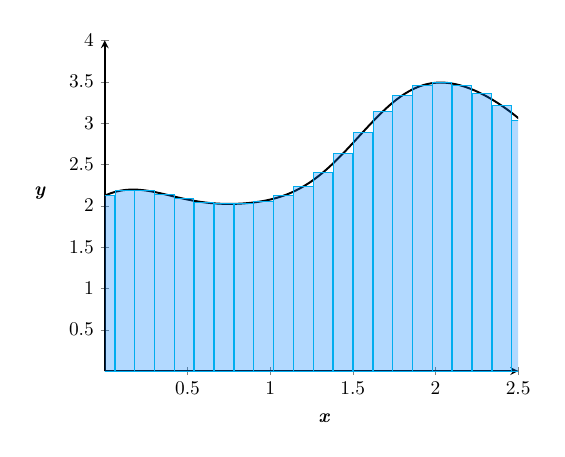
\begin{tikzpicture}[scale=0.7,
    declare function={
    % f(\x)=(\x^2)+9*\x+7;
        f(\x)=2+cos(deg(\x-2))+cos(deg(3*\x))/2+sin(cos(5*\x))/8 + cos(deg(7*\x))/28;
    }
]
\begin{axis}[
    axis lines = middle,
    xtick ={0.5, 1.0, 1.5, 2.0, 2.5, 3.0, 3.5},
    ytick ={0, 0.5, 1, 1.5, 2.0, 2.5, 3, 3.5, 4, 4.5, 5, 5.5},
    % xticklabels = {$a=x_0$,$x_1$,$x_2$,$x_3$, $\ldots$, $x_{n-1}$,$x_n=b$},
    ymin = 0,
    ymax = 4,
    xmin = 0,
    xmax = 2.5,
    x=3cm,y=1.5cm,
    axis line style = thick,
    xlabel style={at={(.5,0)},above right,yshift=-30pt},
    ylabel style={at={(0,.5)},above right,xshift=-40pt},
    xlabel={$\emph{\textbf{x}}$},
    ylabel={$\emph{\textbf{y}}$},
    % extra x ticks={1.3,1.85,2.2,2.7,3.2,3.75}
]

\addplot [
    % domain=1:4,
    samples=300,
    % line width=1pt,
    % fill=red, draw=none,
    % fill opacity=0.1
] {f(x)} \closedcycle;

\addplot [
    domain=0:5,
    samples=300,
    line width = 1pt, black] {f(x)};

\addplot[ybar, bar width=10pt, domain=1:4,samples at={0, 0.12, 0.24, 0.36, 0.48, 0.60, 0.72, 0.84, 0.96, 1.08, 1.20, 1.32, 1.44, 1.56, 1.68, 1.80, 1.92, 2.04, 2.16, 2.28, 2.40, 2.52, 2.64, 2.76, 2.88, 3.00, 3.12, 3.24, 3.36, 3.48}, fill=blue!50!cyan,fill opacity=0.3, draw=cyan]
  {f(x)};
\end{axis}
\end{tikzpicture}
\end{center}
\caption{Midpoint-Riemann Approximation of a Function}
\label{fig:riemannf}
\end{figure}

Design the \ttt{double circleArea(double r, double delta)} method, which receives a radius $r$ and a delta $\Delta$. It computes (and returns) a left/right-Riemann approximation of the area of a circle. Hint: if you compute the left/right-Riemann approximation of one quadrant, you can very easily obtain an approximation of the total circle area. We illustrate this hint in Figure ~\ref{fig:circlearea} where $\Delta=0.5$ and its radius $r=2$. Note that the approximated area will vary based on the chosen Riemann approximation.\footnote{A left-Riemann sum over-approximates the area, whereas a right-Riemann sum provides an under-approximation. A midpoint approximation uses the average between the left and right approximations.} Further note that no calculus knowledge is necessary to solve this exercise.

\begin{figure}[H]
\begin{center}
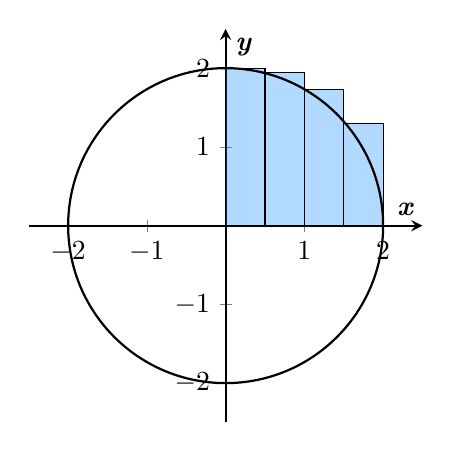
\begin{tikzpicture}
\begin{axis}[
    axis lines = middle,
    xtick ={-3,-2,-1,0,1,2,3},
    ytick ={-3,-2,-1,0,1,2,3},
    % xticklabels = {$a=x_0$,$x_1$,$x_2$,$x_3$, $\ldots$, $x_{n-1}$,$x_n=b$},
    ymin = -2.5,
    ymax = 2.5,
    xmin = -2.5,
    xmax = 2.5,
    x=1cm,y=1cm,
    axis line style = thick,
    xlabel={$\emph{\textbf{x}}$},
    ylabel={$\emph{\textbf{y}}$},
    % extra x ticks={1.3,1.85,2.2,2.7,3.2,3.75}
]
\end{axis}

  \draw[fill=blue!50!cyan,fill opacity=0.3] (2.5,2.5) rectangle (3,4.5);
  \draw[fill=blue!50!cyan,fill opacity=0.3] (3.0,2.5) rectangle (3.5,4.44);
  \draw[fill=blue!50!cyan,fill opacity=0.3] (3.5,2.5) rectangle (4.0,4.23);
  \draw[fill=blue!50!cyan,fill opacity=0.3] (4,2.5) rectangle (4.5,3.80);
\draw[thick] (2.5,2.5) circle (2);
\end{tikzpicture}

\end{center}
\caption{Left-Riemann Approximation of a Function}
\label{fig:circlearea}
\end{figure}

\exercise{3}{chapter-crl}{Speech-to-text software plays a significant role in accessibility for those who may not be able to type quickly or at all. Design the \ttt{String speechToText(String s)} method that, when given a ``speech string', returns the corresponding text. A speech string, in this context, is a string spoken, in English, by a person, which may or may not contain punctuation. If a speech string contains a word that represents punctuation, e.g., \ttt{"period"}, \ttt{"question mark"}, encode this punctuation in the returned text. For example, \ttt{speechToText("hello period how are you question mark")} returns the string \ttt{"Hello. How are you?"}. You should also account for quotations, e.g., \ttt{speechToText\-("hello quote how are you question mark unquote")} returns the string \ttt{Hello. "how are you?"}.}